\begin{frame}[allowframebreaks,allowdisplaybreaks]
    \subsubsection{Keys and Sub-trees}
    \frametitle{B-Tree Properties---Keys and Sub-trees}
    \begin{columns}
        \begin{column}{\textlecolumn}
            \begin{block}{}
                \vspace{-0.8cm}
                \begin{itemize}
                    \item Each key has two sub-trees, one before and one after it. Like a normal tree.
                    \item First, let's define \(N\), a Node which isn't a leaf or \emph{Root}, from a B-Tree.
                    \item Then, we can define the set of the keys on a B-Tree Node \(N\) as \(\left\{k_1, k_2, \ldots{}, k_j\right\}\).
                    \item Leaving the index 0 for a placeholder, which is going to be used later.
                    \item Also, defining \(\symit{l}\) as the number of keys in \(N\).
                    \item Such that for \(t\left(\alpha, h\right)\), we have \(\alpha \leq \symit{l} \leq 2\alpha\).
                \end{itemize}
            \end{block}
        \end{column}
        \begin{column}{\textricolumn}
        \end{column}
    \end{columns}
    \begin{figure}[h!]
        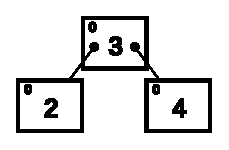
\includegraphics[height=0.175\linewidth]{resources/made/btree_2subtrees.eps}
        \caption{Simple node of a Normal Binary Tree}
    \end{figure}

    \framebreak

    \begin{columns}
        \begin{column}{\textlecolumn}
            \begin{block}{}
                \begin{itemize}
                    \item Now, we also define the set of sub-trees of \(N\) as \(\left\{p_0, p_1, \ldots{}, p_j\right\}\).
                    \item Where \(j\) is the number of sub-trees in \(N\).
                    \item Since there's a sub-tree before and after each key in \(N\).
                    \item Then, \(j\) must be equal to \(\symit{l} + 1\).
                    \item The keys and sub-trees are stored in a sequential increasing order.
                \end{itemize}
            \end{block}
        \end{column}
        \begin{column}{\textricolumn}
        \end{column}
    \end{columns}
    \begin{figure}[h!]
        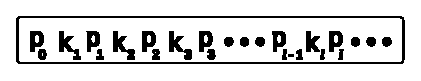
\includegraphics[width=0.85\linewidth]{resources/made/key_subtree_order.eps}
        \caption{Order of the Subtree Pointers and Keys.}
    \end{figure}

    \framebreak

    \begin{columns}
        \begin{column}{\textlecolumn}
            \begin{block}{}
                \begin{itemize}
                    \item In the case that \(N\) is the \emph{Root} of the tree, the only change is the minimum number of keys and sub-trees.
                    \item With \(\symit{l}\), already defined, \emph{Root} will have \(1 \leq \symit{l} \leq 2\alpha\) keys.
                    \item And \(2 \leq \symit{l} + 1 \leq 2\alpha + 1\) sub-trees.
                \end{itemize}
                \begin{itemize}
                    \item If \(N\) is a leaf of the tree, we are going to give the \(k_0\) a simple use.
                    \item The \(k_0\) will store a key value for an object.
                    \item This simple usage on a leaf is just one usage of the \(k_0\) on the nodes.
                \end{itemize}
            \end{block}
        \end{column}
        \begin{column}{\textricolumn}
            \begin{block}{}
            \end{block}
        \end{column}
    \end{columns}
    \begin{figure}
        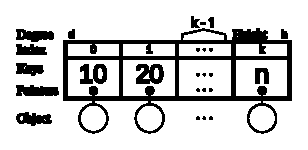
\includegraphics[width=0.45\textwidth]{resources/made/single_leaf.eps}
        \caption[]{Leaf of a B-Tree}
    \end{figure}

    \framebreak

    \begin{columns}
        \begin{column}{\textlecolumn}
            \begin{block}{}
                \begin{itemize}
                    \item Going back where \(N\) is a node on the B-Tree, but now this time \(N\) can be the tree \emph{Root}.
                    \item The order of the keys of \(p_i\), a subtree of \(N\); where \(0 \leq i \leq \symit{l}\), in comparison to the keys of \(N\) can be defined by 3 cases.
                    \item But first, we need to define \(K\left(T\right)\), where \(T \in t\left(\alpha, h\right)\), which is the set of keys inside the Node \(T\).
                    \item And, \(k_j \in K\left(N\right)\), where \(j\) is the index or position of the key in \(N\).
                \end{itemize}
                \vspace{0.5cm}
                \begin{align}
                    \forall y \in K\left(p_0\right);\mspace{20mu}& y < k_1 \tag{Case 1}\label{case1-subt-t-comp} \\
                    \forall y \in K\left(p_{i}\right);\mspace{20mu}& k_i \leq y < k_{i + 1};\mspace{20mu} 0 < i < \symit{l} \wedge i \in \symbb{N} \tag{Case 2}\label{case2-subt-t-comp} \\
                    \forall y \in K\left(p_{\symit{l}}\right);\mspace{20mu}& k_{\symit{l}} \leq y \tag{Case 3}\label{case3-subt-t-comp}
                \end{align}
            \end{block}
        \end{column}
        \begin{column}{\textricolumn}
            \begin{block}{}
            \end{block}
        \end{column}
    \end{columns}
    
    \framebreak

    \begin{columns}
        \begin{column}{0.5\textwidth}
            \begin{figure}
                \centering
                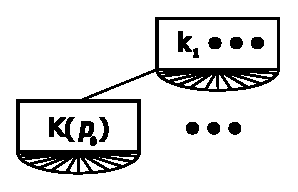
\includegraphics[width=0.55\textwidth]{resources/made/keys_comp_case1.eps}
                \caption{Sub-tree Keys \eqref{case1-subt-t-comp}}
            \end{figure}
        \end{column}
        \begin{column}{0.5\textwidth}
            \begin{figure}
                \centering
                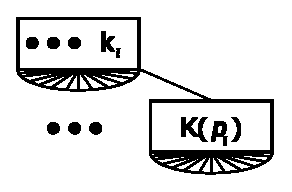
\includegraphics[width=0.55\textwidth]{resources/made/keys_comp_case3.eps}
                \caption{Sub-tree Keys \eqref{case3-subt-t-comp}}
            \end{figure}
        \end{column}
    \end{columns}
    \begin{figure}
        \centering
        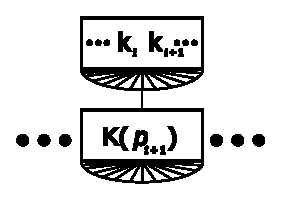
\includegraphics[width=0.3\textwidth]{resources/made/keys_comp_case2.eps}
        \caption{Sub-tree Keys \eqref{case2-subt-t-comp}}
    \end{figure}
\end{frame}
